%
% einleitung.tex -- Beispiel-File für die Einleitung
%
% (c) 2020 Prof Dr Andreas Müller, Hochschule Rapperswil
%
\section{Modellierung von Populationen
\label{logistic:section:einleitung}}
\rhead{Modellierung von Populationen}

Die logistische Gleichung ist ein beliebtes mathematisches Objekt,
das zeigt, wie aus einer scheinbar einfach Gleichung
ein sehr komplexes und chaotisches Verhalten entstehen kann. 
Ihren Urpsrung hat die logistische Gleichung beim Modellieren
vom zeitlichen Verlauf von Populationen. 
Wie man dabei ganz organisch auf die logistische Gleichung 
kommt, wird in diesem Abschnitt kurz demonstriert. 

Als Erstes nehmen wir eine Population an, 
die ungehindert wachsen kann. 
Anfänglich hat diese die Tendenz, exponentiell zu wachsen. 
In Gleichung \eqref{eq:lambda_xn} ist $x_{n}$ die Population zu einem bestimmten Zeitpunkt, 
beispielsweise am Anfang vom Jahr $n$. 
Nun ist $x_{n+1}$ die Population im darauf folgenden Jahr, 
welche damit eine direkte Funktion der Population im vorherigen
Jahr ist. 
Ein einfaches mathematisches Modell für dieses Verhalten
könnte wie folgt aussehen:
\begin{equation}
    \label{eq:lambda_xn}
    x_{n+1} = \lambda x_{n}\text{.}
\end{equation}
Der Faktor $\lambda$ gibt in diesem Modell an, 
wie schnell die Population von Jahr zu Jahr ansteigt. 
Es ist schnell erkennbar, 
dass ein $\lambda > 1$ ein Wachstum und
ein $\lambda < 1$ einen Zerfall
der Population im folgenden Jahr zur Folge hat. 
Abbildung \ref{fig:pop_exp} zeigt die jährlichen
Entwicklungen von Populationen für verschiedene
Werte von $\lambda$ mit diesem Modell.
Auf der linken Grafik mit $\lambda = 0.75$ ist deutlich
ein exponentieller Zerfall und auf 
der rechten Grafik mit $\lambda = 1.25$
ein exponentielles Wachstum ersichtlich.
\begin{figure}
    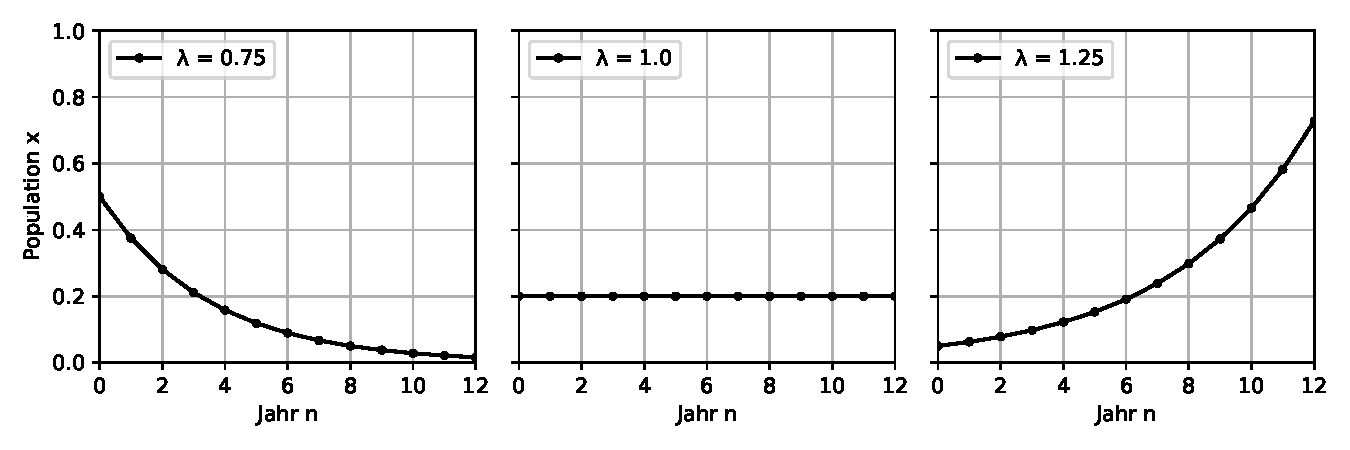
\includegraphics[width=\linewidth]{papers/logistic/figures/pop_exp.pdf}
    \caption{
        Exponentielle Populationsverläufe nach
        Gleichung \eqref{eq:lambda_xn}
        und verschiedenen Werten von $\lambda$.
    }
    \label{fig:pop_exp}
\end{figure}

In der Realität können Populationen natürlich nicht endlos
exponentiell weiterwachsen, 
da früher oder später Platz, Nahrung, usw. ausgehen.
Um dieses Verhalten in das Modell zu implementieren,
fügen wir noch einen zusätzlichen Term hinzu, 
womit wir auch schon bei der logistischen Gleichung 
\begin{equation}
    \label{eq:logistic}
    x_{n+1} = \lambda x_{n} (1 - x_{n})
\end{equation}
angekommen sind.
Dieser neue Term sorgt dafür, 
dass das Wachstum der Population zurückgeht, 
wenn sie grösser wird.
Der Wert von $x_n$ ist so limitiert auf 
$0 \le x_n \le 1$  
und kann als die relative Population mit einem
theoretischen Maximum von 1 interpretiert werden. 
Abbildung \ref{fig:pop_logistic} zeigt nun
für einige Werte von $\lambda$\
die jährlichen Entwicklungen von Populationen 
welche mit der logistischen Gleichung modelliert werden.
Dazu ist zum Vergleich das bereits bekannte exponentielle Modell
mit gleichem $\lambda$ als gestrichelte Linie abgebildet. 
Auf der linken Grafik ist auch hier wieder erkennbar, 
dass ein $\lambda < 1$ zur Folge hat, 
dass die Population rasch ausstirbt. 
Auf der mittleren Grafik mit $\lambda = 1.8$ sieht 
die Kurve zuerst annähernd exponentiell wachsend aus,
doch der neu hinzugefügte Term sorgt jetzt dafür, 
dass das Wachstum bei grösser werdender Population zurückgeht 
und sich schliesslich auf $\approx 0.42$ einpendelt. 
Sehr interessant ist die rechten Grafik mit $\lambda = 2.8$,
wo die Population zuerst ein wenig ``überschwingt'', 
sich aber schliesslich auf $\approx 0.62$ einpendelt.  
\begin{figure}
    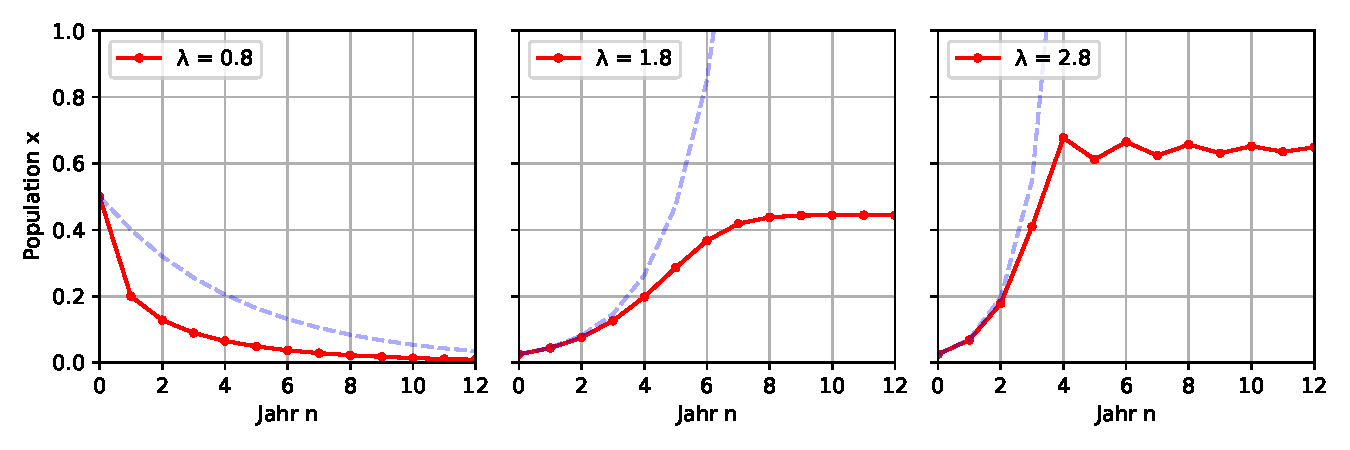
\includegraphics[width=\linewidth]{papers/logistic/figures/pop_logistic.pdf}
    \caption{
        In rot:
        logistische Populationsverläufe nach
        Gleichung \eqref{eq:logistic} und
        verschiedenen Werten von $\lambda$.
        In blau, zum Vergleich:
        exponentielle Populationsverläufe nach 
        Gleichung \eqref{eq:lambda_xn} mit gleichem $\lambda$.
    }
    \label{fig:pop_logistic}
\end{figure}